\documentclass[twoside]{book}

% Packages required by doxygen
\usepackage{fixltx2e}
\usepackage{calc}
\usepackage{doxygen}
\usepackage[export]{adjustbox} % also loads graphicx
\usepackage{graphicx}
\usepackage[utf8]{inputenc}
\usepackage{makeidx}
\usepackage{multicol}
\usepackage{multirow}
\PassOptionsToPackage{warn}{textcomp}
\usepackage{textcomp}
\usepackage[nointegrals]{wasysym}
\usepackage[table]{xcolor}

% Font selection
\usepackage[T1]{fontenc}
\usepackage[scaled=.90]{helvet}
\usepackage{courier}
\usepackage{amssymb}
\usepackage{sectsty}
\renewcommand{\familydefault}{\sfdefault}
\allsectionsfont{%
  \fontseries{bc}\selectfont%
  \color{darkgray}%
}
\renewcommand{\DoxyLabelFont}{%
  \fontseries{bc}\selectfont%
  \color{darkgray}%
}
\newcommand{\+}{\discretionary{\mbox{\scriptsize$\hookleftarrow$}}{}{}}

% Page & text layout
\usepackage{geometry}
\geometry{%
  a4paper,%
  top=2.5cm,%
  bottom=2.5cm,%
  left=2.5cm,%
  right=2.5cm%
}
\tolerance=750
\hfuzz=15pt
\hbadness=750
\setlength{\emergencystretch}{15pt}
\setlength{\parindent}{0cm}
\setlength{\parskip}{3ex plus 2ex minus 2ex}
\makeatletter
\renewcommand{\paragraph}{%
  \@startsection{paragraph}{4}{0ex}{-1.0ex}{1.0ex}{%
    \normalfont\normalsize\bfseries\SS@parafont%
  }%
}
\renewcommand{\subparagraph}{%
  \@startsection{subparagraph}{5}{0ex}{-1.0ex}{1.0ex}{%
    \normalfont\normalsize\bfseries\SS@subparafont%
  }%
}
\makeatother

% Headers & footers
\usepackage{fancyhdr}
\pagestyle{fancyplain}
\fancyhead[LE]{\fancyplain{}{\bfseries\thepage}}
\fancyhead[CE]{\fancyplain{}{}}
\fancyhead[RE]{\fancyplain{}{\bfseries\leftmark}}
\fancyhead[LO]{\fancyplain{}{\bfseries\rightmark}}
\fancyhead[CO]{\fancyplain{}{}}
\fancyhead[RO]{\fancyplain{}{\bfseries\thepage}}
\fancyfoot[LE]{\fancyplain{}{}}
\fancyfoot[CE]{\fancyplain{}{}}
\fancyfoot[RE]{\fancyplain{}{\bfseries\scriptsize Generated by Doxygen }}
\fancyfoot[LO]{\fancyplain{}{\bfseries\scriptsize Generated by Doxygen }}
\fancyfoot[CO]{\fancyplain{}{}}
\fancyfoot[RO]{\fancyplain{}{}}
\renewcommand{\footrulewidth}{0.4pt}
\renewcommand{\chaptermark}[1]{%
  \markboth{#1}{}%
}
\renewcommand{\sectionmark}[1]{%
  \markright{\thesection\ #1}%
}

% Indices & bibliography
\usepackage{natbib}
\usepackage[titles]{tocloft}
\setcounter{tocdepth}{3}
\setcounter{secnumdepth}{5}
\makeindex

% Hyperlinks (required, but should be loaded last)
\usepackage{ifpdf}
\ifpdf
  \usepackage[pdftex,pagebackref=true]{hyperref}
\else
  \usepackage[ps2pdf,pagebackref=true]{hyperref}
\fi
\hypersetup{%
  colorlinks=true,%
  linkcolor=blue,%
  citecolor=blue,%
  unicode%
}

% Custom commands
\newcommand{\clearemptydoublepage}{%
  \newpage{\pagestyle{empty}\cleardoublepage}%
}

\usepackage{caption}
\captionsetup{labelsep=space,justification=centering,font={bf},singlelinecheck=off,skip=4pt,position=top}

%===== C O N T E N T S =====

\begin{document}

% Titlepage & ToC
\hypersetup{pageanchor=false,
             bookmarksnumbered=true,
             pdfencoding=unicode
            }
\pagenumbering{roman}
\begin{titlepage}
\vspace*{7cm}
\begin{center}%
{\Large Usporiadane procesy }\\
\vspace*{1cm}
{\large Generated by Doxygen 1.8.11}\\
\end{center}
\end{titlepage}
\clearemptydoublepage
\tableofcontents
\clearemptydoublepage
\pagenumbering{arabic}
\hypersetup{pageanchor=true}

%--- Begin generated contents ---
\chapter{Class Index}
\section{Class List}
Here are the classes, structs, unions and interfaces with brief descriptions\+:\begin{DoxyCompactList}
\item\contentsline{section}{\hyperlink{struct__App}{\+\_\+\+App} \\*Pseudo-\/objekt specifikacia atributov }{\pageref{struct__App}}{}
\item\contentsline{section}{\hyperlink{struct__Front}{\+\_\+\+Front} \\*Pseudo-\/objekt specifikacia atributov }{\pageref{struct__Front}}{}
\item\contentsline{section}{\hyperlink{struct__Matica}{\+\_\+\+Matica} \\*Pseudo-\/objekt specifikuje atributy }{\pageref{struct__Matica}}{}
\item\contentsline{section}{\hyperlink{struct__Proces}{\+\_\+\+Proces} }{\pageref{struct__Proces}}{}
\end{DoxyCompactList}

\chapter{Class Documentation}
\hypertarget{struct__App}{}\section{\+\_\+\+App Struct Reference}
\label{struct__App}\index{\+\_\+\+App@{\+\_\+\+App}}


Pseudo-\/objekt specifikacia atributov.  




{\ttfamily \#include $<$App.\+h$>$}

\subsection*{Public Attributes}
\begin{DoxyCompactItemize}
\item 
const char $\ast$ \hyperlink{struct__App_a75b8ceb6c793d2eafac8395c13fc0b0a}{nazov\+\_\+suboru}
\end{DoxyCompactItemize}


\subsection{Detailed Description}
Pseudo-\/objekt specifikacia atributov. 

Reprezentuje instanciu aplikacie 

\subsection{Member Data Documentation}
\index{\+\_\+\+App@{\+\_\+\+App}!nazov\+\_\+suboru@{nazov\+\_\+suboru}}
\index{nazov\+\_\+suboru@{nazov\+\_\+suboru}!\+\_\+\+App@{\+\_\+\+App}}
\subsubsection[{\texorpdfstring{nazov\+\_\+suboru}{nazov_suboru}}]{\setlength{\rightskip}{0pt plus 5cm}const char$\ast$ \+\_\+\+App\+::nazov\+\_\+suboru}\hypertarget{struct__App_a75b8ceb6c793d2eafac8395c13fc0b0a}{}\label{struct__App_a75b8ceb6c793d2eafac8395c13fc0b0a}
Nazov vstupneho suboru s orientovanym grafom. 

The documentation for this struct was generated from the following file\+:\begin{DoxyCompactItemize}
\item 
/home/katka/\+Documents/\+O\+S\+\_\+usporiadane\+Procesy/src/\hyperlink{App_8h}{App.\+h}\end{DoxyCompactItemize}

\hypertarget{struct__Front}{}\section{\+\_\+\+Front Struct Reference}
\label{struct__Front}\index{\+\_\+\+Front@{\+\_\+\+Front}}
\subsection*{Public Attributes}
\begin{DoxyCompactItemize}
\item 
void $\ast$$\ast$ {\bfseries pole}\hypertarget{struct__Front_aaeb70caeedb19e72ba106f621e496942}{}\label{struct__Front_aaeb70caeedb19e72ba106f621e496942}

\item 
size\+\_\+t {\bfseries poc\+\_\+prkov}\hypertarget{struct__Front_a4eadefd147ef83ec0a5f855046ad192a}{}\label{struct__Front_a4eadefd147ef83ec0a5f855046ad192a}

\item 
int {\bfseries akt\+\_\+pozicia\+\_\+pop}\hypertarget{struct__Front_ab755728649fe43c6e3c394ed168387d7}{}\label{struct__Front_ab755728649fe43c6e3c394ed168387d7}

\item 
int {\bfseries akt\+\_\+pozicia\+\_\+push}\hypertarget{struct__Front_a0931c8786584f8671ec4b7c42ba2bdee}{}\label{struct__Front_a0931c8786584f8671ec4b7c42ba2bdee}

\end{DoxyCompactItemize}


The documentation for this struct was generated from the following file\+:\begin{DoxyCompactItemize}
\item 
/home/katka/\+Documents/\+O\+S\+\_\+usporiadane\+Procesy/src/Front.\+h\end{DoxyCompactItemize}

\hypertarget{struct__Matica}{}\section{\+\_\+\+Matica Struct Reference}
\label{struct__Matica}\index{\+\_\+\+Matica@{\+\_\+\+Matica}}
\subsection*{Public Attributes}
\begin{DoxyCompactItemize}
\item 
int $\ast$$\ast$ {\bfseries pole}\hypertarget{struct__Matica_ac3fca0017962cbf096d0e50b54c640b0}{}\label{struct__Matica_ac3fca0017962cbf096d0e50b54c640b0}

\item 
size\+\_\+t {\bfseries velkost\+\_\+strany}\hypertarget{struct__Matica_a089eec293e9332883a0a8963043ae869}{}\label{struct__Matica_a089eec293e9332883a0a8963043ae869}

\end{DoxyCompactItemize}


The documentation for this struct was generated from the following file\+:\begin{DoxyCompactItemize}
\item 
/home/katka/\+Documents/\+O\+S\+\_\+usporiadane\+Procesy/src/Matica.\+h\end{DoxyCompactItemize}

\hypertarget{struct__Proces}{}\section{\+\_\+\+Proces Struct Reference}
\label{struct__Proces}\index{\+\_\+\+Proces@{\+\_\+\+Proces}}


Collaboration diagram for \+\_\+\+Proces\+:\nopagebreak
\begin{figure}[H]
\begin{center}
\leavevmode
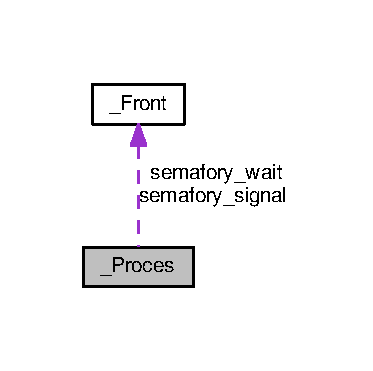
\includegraphics[width=179pt]{struct__Proces__coll__graph}
\end{center}
\end{figure}
\subsection*{Public Attributes}
\begin{DoxyCompactItemize}
\item 
sem\+\_\+t $\ast$ {\bfseries semafor}\hypertarget{struct__Proces_ae861d8129ec67d9e340f035f371d0d1d}{}\label{struct__Proces_ae861d8129ec67d9e340f035f371d0d1d}

\item 
int {\bfseries koeficient}\hypertarget{struct__Proces_adc9eff4877d9e51470d0a9c386b00c40}{}\label{struct__Proces_adc9eff4877d9e51470d0a9c386b00c40}

\item 
\hyperlink{Front_8h_aeda6f9a18e68a801590717ec948afc22}{Front} $\ast$ {\bfseries semafory\+\_\+wait}\hypertarget{struct__Proces_a084d71b0a72065a85df0f51e9b1b3107}{}\label{struct__Proces_a084d71b0a72065a85df0f51e9b1b3107}

\item 
\hyperlink{Front_8h_aeda6f9a18e68a801590717ec948afc22}{Front} $\ast$ {\bfseries semafory\+\_\+signal}\hypertarget{struct__Proces_acb70bd09f8b74c247a3040236a35c2f3}{}\label{struct__Proces_acb70bd09f8b74c247a3040236a35c2f3}

\end{DoxyCompactItemize}


The documentation for this struct was generated from the following file\+:\begin{DoxyCompactItemize}
\item 
/home/katka/\+Documents/\+O\+S\+\_\+usporiadane\+Procesy/src/\hyperlink{App_8c}{App.\+c}\end{DoxyCompactItemize}

%--- End generated contents ---

% Index
\backmatter
\newpage
\phantomsection
\clearemptydoublepage
\addcontentsline{toc}{chapter}{Index}
\printindex

\end{document}
